\documentclass[aspectratio=169]{beamer}

\usepackage{ccicons}
\usepackage{fontspec}
\usepackage{listings}
\usepackage{tikz}
\usepackage{svg}

\definecolor{uclablue}{RGB}{39,116,174}
\definecolor{uclagold}{RGB}{255,179,0}

\definecolor{ubcorange}{RGB}{158, 66, 37}

\definecolor{cugold}{RGB}{207, 184, 124}
\definecolor{cudarkgray}{RGB}{86, 90, 92}

\definecolor{solarizedred}{RGB}{220, 50, 47}
\definecolor{solarizedblue}{RGB}{38, 139, 210}
\definecolor{solarizedgreen}{RGB}{133, 153, 0}
\definecolor{solarizedpurple}{RGB}{108, 113, 196}
\definecolor{solarizedmagenta}{RGB}{211, 54, 130}

\definecolor{pantone655}{RGB}{0, 42, 92}
\definecolor{pantone7453}{RGB}{123, 164, 217}
\definecolor{pantone633}{RGB}{0, 139, 176}
\definecolor{pantone7492}{RGB}{218, 229, 205}

\colorlet{primarycolor}{pantone655}
\colorlet{secondarycolor}{pantone7453}


\usetikzlibrary{
  arrows,
  arrows.meta,
  automata,
  backgrounds,
  calc,
  chains,
  decorations.pathreplacing,
  fit,
  intersections,
  matrix,
  overlay-beamer-styles,
  positioning,
  shapes,
  shapes.multipart,
  tikzmark,
}
\usetikzmarklibrary{listings}

\hypersetup{
  colorlinks=true,
  urlcolor=cudarkgray,
}

\setbeamercolor{frametitle}{fg=primarycolor}
\setbeamercolor{structure}{fg=primarycolor}
\setbeamercolor{enumerate item}{fg=black}
\setbeamercolor{itemize item}{fg=black}
\setbeamercolor{itemize subitem}{fg=black}

\setbeamersize{text margin left=26.6mm}
\addtolength{\headsep}{2mm}

\setbeamertemplate{navigation symbols}{}
\setbeamertemplate{headline}{}
\setbeamertemplate{footline}{}
\setbeamertemplate{itemize item}{\color{black}}
\setbeamertemplate{itemize items}[circle]

\setbeamertemplate{footline}{
  \begin{tikzpicture}[remember picture,
                      overlay,
                      shift={(current page.south west)}]
    \node [black!50, inner sep=2mm, anchor=south east]
          at (current page.south east) {\footnotesize \insertframenumber};
  \end{tikzpicture}
}

\setsansfont{Inter}[Scale=MatchLowercase]
\setmonofont{Hack}[Scale=MatchLowercase]

\makeatletter
\newcommand\version[1]{\renewcommand\@version{#1}}
\newcommand\@version{}
\def\insertversion{\@version}

\newcommand\lecturenumber[1]{\renewcommand\@lecturenumber{#1}}
\newcommand\@lecturenumber{}
\def\insertlecturenumber{\@lecturenumber}
\makeatother

\setbeamertemplate{title page}
{
  \begin{tikzpicture}[remember picture,
                      overlay,
                      shift={(current page.south west)},
                      background rectangle/.style={fill=pantone655},
                      show background rectangle]
    \node [anchor=west, align=left, inner sep=0, text=white]
          (lecturenumber) at (\paperwidth / 6, \paperheight * 3 / 4)
          {\Large Lecture \insertlecturenumber};
    \node [inner sep=0, align=left, text=white, node distance=0,
          above left=of lecturenumber, anchor=south west, yshift=2mm]
          {\Large ECE 344: Operating Systems};
    \node (title) [inner sep=0, anchor=west, align=left, text=white,
                   text width=30em]
          at (\paperwidth / 6, \paperheight / 2)
          {{\bfseries \Huge \inserttitle{}}};
    \node [inner sep=0, align=right, text=white, node distance=0,
          below right=of title, anchor=north east, yshift=-1mm]
          {{\footnotesize \ttfamily \insertversion}};
    \node [inner sep=0, text=white, align=left, anchor=west]
          (author) at (\paperwidth / 6, \paperheight / 4)
          {\insertauthor};
    \node [text=white, inner sep=0, align=left, node distance=0,
           below left=of author, anchor=north west, yshift=-2mm]
          {\insertdate};
    \node [align=right, anchor=south east, inner sep=2mm, text=white]
          (license) at (\paperwidth, 0)
          {\footnotesize This  work is licensed under a
           \href{http://creativecommons.org/licenses/by-sa/4.0/}
                {\color{pantone7453} Creative Commons Attribution-ShareAlike 4.0
                 International License}};
    \node [text=white, inner sep=0, align=right, node distance=0,
           above right=of license, anchor=south east, xshift=-2mm]
          {\Large \ccbysa};
  \end{tikzpicture}
}

\tikzset{
  >=Straight Barb[],
  shorten >=1pt,
  initial text=,
}

\lstset{
  basicstyle=\footnotesize\ttfamily,
  language=C,
  escapechar=@,
  commentstyle=\color{black!50},
}


\lecturenumber{24}
\title{Basic Memory Allocation}
\version{1.0.0}
\author{Jon Eyolfson}
\date{November 14, 2022}

\begin{document}
  \begin{frame}[plain, noframenumbering]
    \titlepage
  \end{frame}

  \begin{frame}
    \frametitle{Static Allocation is the Simplest Strategy}

    Create a fixed size allocation in your program

    \hspace{2em} e.g. \lstinline|char buffer[4096];|

    \vspace{2em}

    When the program loads, the kernel sets aside that memory
    for you

    \vspace{2em}

    That memory exists as long as your process does, no need to free
  \end{frame}

  \begin{frame}
    \frametitle{Dynamic Allocation is Often Required}

    You may only conditionally require memory

    \hspace{2em} Static allocations are sometimes wasteful

    \vspace{2em}

    You may not know the size of the allocation

    \hspace{2em} Static allocations need to account for the maximum size

    \vspace{2em}

    Where do you allocate memory?

    \hspace{2em} You can either allocate on the stack or on the heap
  \end{frame}

  \begin{frame}
    \frametitle{Stack Allocation is Mostly Done for You in C}

    Think of normal variables

    \hspace{2em} e.g. \lstinline|int x;|

    \vspace{2em}

    The compiler internally inserts \lstinline|alloca| calls

    \hspace{2em} e.g. \lstinline|int *px = (int*) alloca(4);|

    \vspace{2em}

    Whenever the function that called \lstinline|alloca| returns, it
    frees all the memory

    \hspace{2em} This just restores the previous stack pointer

    \vspace{2em}

    This won't work if you try to use the memory after returning
  \end{frame}

  \begin{frame}
    \frametitle{You've Used Dynamic Allocation Before}

    These are the \lstinline|malloc| family of functions

    \vspace{2em}

    The most flexible way to use memory, but is also the most difficult to get
    right

    \vspace{2em}

    You have to properly handle your memory lifetimes, and \lstinline|free|
    exactly once

    \vspace{2em}

    Also, there's a new concern --- fragmentation
  \end{frame}

  \begin{frame}
    \frametitle{Fragmentation is a Unique Issue for Dynamic Allocation}

    You allocate memory in different sized contiguous blocks

    \hspace{2em} Compaction is not possible and every allocation decision is
    permanent

    \vspace{2em}

    A fragment is a small contiguous block of memory that cannot handle an allocation

    \hspace{2em} You can think of it as a ``hole'' in memory, wasting space

    \vspace{2em}

    There are 3 requirements for fragmentation
    \begin{enumerate}
        \item Different allocation lifetimes
        \item Different allocation sizes
        \item Inability to relocate previous allocations  
    \end{enumerate}
  \end{frame}

  \begin{frame}{There's Internal and External Fragmentation}

    External fragmentation occurs when you allocate different sized blocks

    \hspace{2em} There's no room for an allocation between the blocks

    \begin{center}
    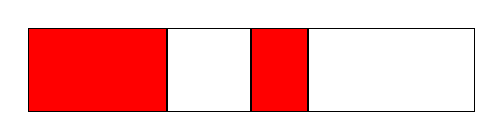
\begin{tikzpicture}[node distance=0mm and 0mm]
      \node[draw,rectangle,minimum width=50,minimum height=30,fill=red]
        (a0) {};
      \node[draw,rectangle,minimum width=30,minimum height=30]
        (a1) [right=of a0] {};
      \node[draw,rectangle,minimum width=20,minimum height=30,fill=red]
        (a2) [right=of a1] {};
      \node[draw,rectangle,minimum width=60,minimum height=30]
        (a3) [right=of a2] {};
    \end{tikzpicture}
    \end{center}

    Internal fragmentation occurs when you allocate fixed sized blocks

    \hspace{2em} There's wasted space within a block

    \begin{center}
    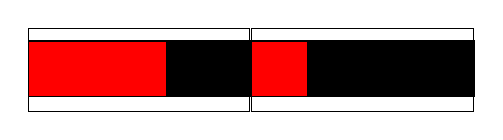
\begin{tikzpicture}[node distance=0mm and 0mm]
      \node[draw,rectangle,minimum width=50,minimum height=20,fill=red]
        (a0) {};
      \node[draw,rectangle,minimum width=30,minimum height=20,fill=black]
        (a1) [right=of a0] {};
      \node[draw,rectangle,minimum width=20,minimum height=20,fill=red]
        (a2) [right=of a1] {};
      \node[draw,rectangle,minimum width=60,minimum height=20,fill=black]
        (a3) [right=of a2] {};
      \node[draw,rectangle,minimum width=80,minimum height=30,xshift=15,yshift=25]
        [below=of a0] {};
      \node[draw,rectangle,minimum width=80,minimum height=30,xshift=30,yshift=25]
        [below=of a2] {};
    \end{tikzpicture}
    \end{center}

    \begin{flushright}
      Credit: \href{https://git.scc.kit.edu/uurqi/os-tutorium}{Daniel Ritz}
    \end{flushright}
  \end{frame}

  \begin{frame}
    \frametitle{We Want to Minimize Fragmentation}

    Fragmentation is just wasted space, which we should prevent

    \vspace{2em}

    We want to reduce the number of ``holes'' between blocks of memory

    \hspace{2em} If we have holes, we'd like to keep them as large as possible

    \vspace{2em}

    Our goal is to keep allocating memory without wasting space
  \end{frame}

  \begin{frame}
    \frametitle{Allocator Implementations Usually Use a Free List}

    They keep track of free blocks of memory by chaining them together

    \hspace{2em} Implemented with a linked list

    \vspace{2em}

    We need to be able to handle a request of any size

    \vspace{2em}

    For allocation, we choose a block large enough for the request

    \hspace{2em} Remove it from the free list

    \vspace{2em}

    For deallocation, we add the block back to the free list

    \hspace{2em} If it's adjacent to another free block, we can merge them
  \end{frame}

  \begin{frame}
    \frametitle{There are 3 General Heap Allocation Strategies}

    Best fit: choose the smallest block that can satisfy the request

    \hspace{2em} Needs to search through the whole list (unless there's an
    exact match)

    \vspace{2em}

    Worst fit: choose largest block (most leftover space)

    \hspace{2em} Also has to search through the list

    \vspace{2em}
    
    First fit: choose first block that can satisfy request
  \end{frame}

  \begin{frame}{Allocating Using Best Fit (1)}

    Note that blocks with a blank background and a number are free

    \vspace{2em}

    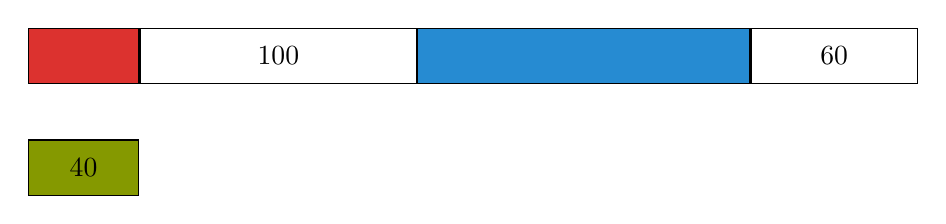
\begin{tikzpicture}[node distance=0mm and 0mm]
      \node[draw,rectangle,minimum width=40,minimum height=20,fill=solarizedred]
        (a0) {};
      \node[draw,rectangle,minimum width=100,minimum height=20]    (a1)  [right=of a0]      {100};
      \node[draw,rectangle,minimum width=120,minimum height=20,fill=solarizedblue]    (a2) [right=of a1]       {};
      \node[draw,rectangle,minimum width=60,minimum height=20]    (a3)    [right=of a2]    {60};

      \node[draw,rectangle,minimum width=40,minimum height=20,yshift=-20,fill=solarizedgreen]
        [below=of a0] {40};
    \end{tikzpicture}

    Where do we allocate this block?
  \end{frame}

  \begin{frame}{Allocating Using Best Fit (2)}
    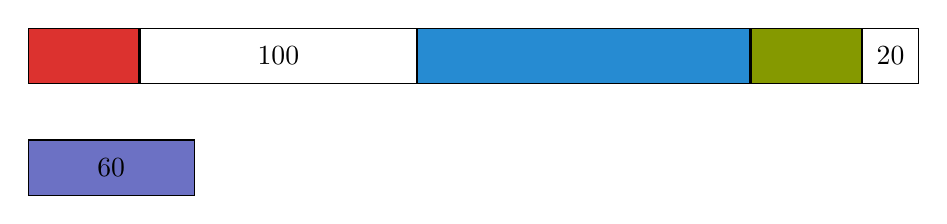
\begin{tikzpicture}[node distance=0mm and 0mm]
            
      \node[draw,rectangle,minimum width=40,minimum height=20,fill=solarizedred]    (a0)        {};
      \node[draw,rectangle,minimum width=100,minimum height=20]    (a1)  [right=of a0]      {100};
      \node[draw,rectangle,minimum width=120,minimum height=20,fill=solarizedblue]    (a2) [right=of a1]       {};
      \node[draw,rectangle,minimum width=40,minimum height=20,fill=solarizedgreen]    (a3)    [right=of a2]    {};
      \node[draw,rectangle,minimum width=20,minimum height=20]    (a4)    [right=of a3]    {20};

      \node[draw,rectangle,minimum width=60,minimum height=20,yshift=-20,xshift=10,fill=solarizedpurple] [below=of a0] {60};

    \end{tikzpicture}

    Where do we allocate this block?
  \end{frame}

  \begin{frame}{Allocating Using Best Fit (3)}
    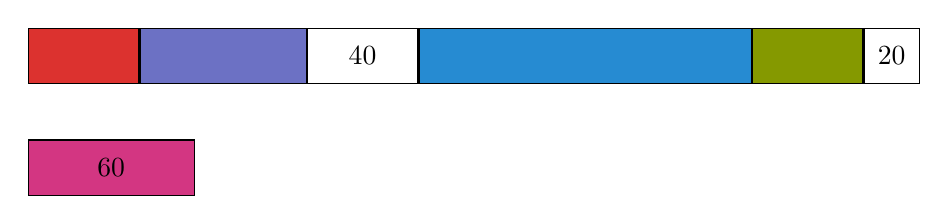
\begin{tikzpicture}[node distance=0mm and 0mm]
      \node[draw,rectangle,minimum width=40,minimum height=20,fill=solarizedred]    (a0)        {};
      \node[draw,rectangle,minimum width=60,minimum height=20,fill=solarizedpurple]    (a1)  [right=of a0]      {};
      \node[draw,rectangle,minimum width=40,minimum height=20]    (a2)  [right=of a1]      {40};
      \node[draw,rectangle,minimum width=120,minimum height=20,fill=solarizedblue]    (a3) [right=of a2]       {};
      \node[draw,rectangle,minimum width=40,minimum height=20,fill=solarizedgreen]    (a4)    [right=of a3]    {};
      \node[draw,rectangle,minimum width=20,minimum height=20]    (a5)    [right=of a4]    {20};

      \node[draw,rectangle,minimum width=60,minimum height=20,yshift=-20,xshift=10,fill=solarizedmagenta] [below=of a0] {60};
    \end{tikzpicture}

    The next block does not fit anywhere
  \end{frame}

  \begin{frame}{Allocating Using Worst Fit (1)}
    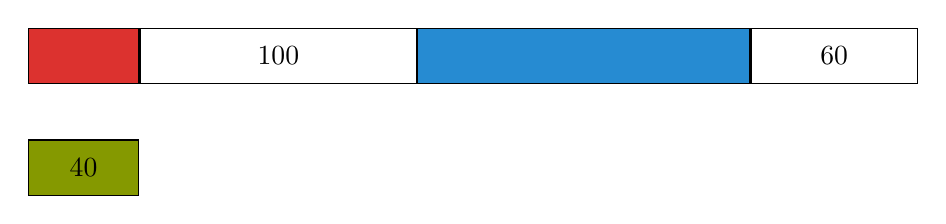
\begin{tikzpicture}[node distance=0mm and 0mm]
        \node[draw,rectangle,minimum width=40,minimum height=20,fill=solarizedred]    (a0)        {};
        \node[draw,rectangle,minimum width=100,minimum height=20]    (a1)  [right=of a0]      {100};
        \node[draw,rectangle,minimum width=120,minimum height=20,fill=solarizedblue]    (a2) [right=of a1]       {};
        \node[draw,rectangle,minimum width=60,minimum height=20]    (a3)    [right=of a2]    {60};

        \node[draw,rectangle,minimum width=40,minimum height=20,yshift=-20,fill=solarizedgreen] [below=of a0] {40};
    \end{tikzpicture}

    Where do we allocate this block?
  \end{frame}

  \begin{frame}{Allocating Using Worst Fit (2)}
    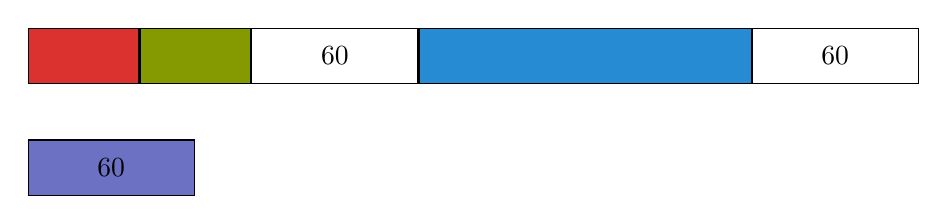
\begin{tikzpicture}[node distance=0mm and 0mm]
        \node[draw,rectangle,minimum width=40,minimum height=20,fill=solarizedred]    (a0)        {};
        \node[draw,rectangle,minimum width=40,minimum height=20,fill=solarizedgreen]    (a1)  [right=of a0]      {};
        \node[draw,rectangle,minimum width=60,minimum height=20]    (a2)    [right=of a1]    {60};
        \node[draw,rectangle,minimum width=120,minimum height=20,fill=solarizedblue]    (a3) [right=of a2]       {};
        \node[draw,rectangle,minimum width=60,minimum height=20]    (a4)    [right=of a3]    {60};

        \node[draw,rectangle,minimum width=60,minimum height=20,yshift=-20,xshift=10,fill=solarizedpurple] [below=of a0] {60};
    \end{tikzpicture}

    Where do we allocate this block?
  \end{frame}

  \begin{frame}{Allocating Using Worst Fit (3)}
    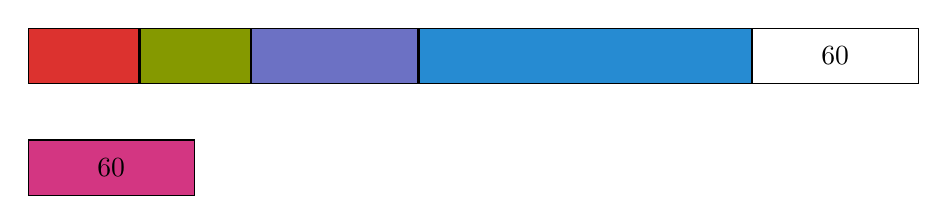
\begin{tikzpicture}[node distance=0mm and 0mm]
        \node[draw,rectangle,minimum width=40,minimum height=20,fill=solarizedred]    (a0)        {};
        \node[draw,rectangle,minimum width=40,minimum height=20,fill=solarizedgreen]    (a1)  [right=of a0]      {};
        \node[draw,rectangle,minimum width=60,minimum height=20,fill=solarizedpurple]    (a2)    [right=of a1]    {};
        \node[draw,rectangle,minimum width=120,minimum height=20,fill=solarizedblue]    (a3) [right=of a2]       {};
        \node[draw,rectangle,minimum width=60,minimum height=20]    (a4)    [right=of a3]    {60};

        \node[draw,rectangle,minimum width=60,minimum height=20,yshift=-20,xshift=10,fill=solarizedmagenta] [below=of a0] {60};
    \end{tikzpicture}

    Next block fits exactly in remaining space
  \end{frame}

  \begin{frame}
    \frametitle{Best Fit and Worst Fit are Both Slow}

    Best fit: tends to leave very large holes and very small holes

    \hspace{2em} Small holes may be useless

    \vspace{2em}

    Worst fit: simulation says it's the worst in terms of storage utilization

    \vspace{2em}

    First fit: tends to leave ``average'' size holes
  \end{frame}

  \begin{frame}
    \frametitle{The Kernel Has To Implement It's Own Memory Allocations}

    The concepts are the same for user space memory allocation

    (the kernel just gives them more contiguous virtual memory pages):

    \begin{itemize}
      \item There's static and dynamic allocations
      \item For dynamic allocations, fragmentation is a big concern
      \item Dynamic allocation returns blocks of memory
        \begin{itemize}
          \item Fragmentation between blocks is external
          \item Fragmentation within a blocks is internal
        \end{itemize}
      \item There's 3 general allocation strategies for different sized
            allocations
        \begin{itemize}
          \item Best fit
          \item Worst fit
          \item First fit
        \end{itemize}
    \end{itemize}
  \end{frame}
\end{document}
